
%title page
\begin{frame}
\titlepage
\end{frame}

\section{Introduction}

\begin{frame}{Big data in astroparticle physics (APP)}
    \small
    \begin{minipage}[c]{0.58\textwidth}
        \begin{center}
            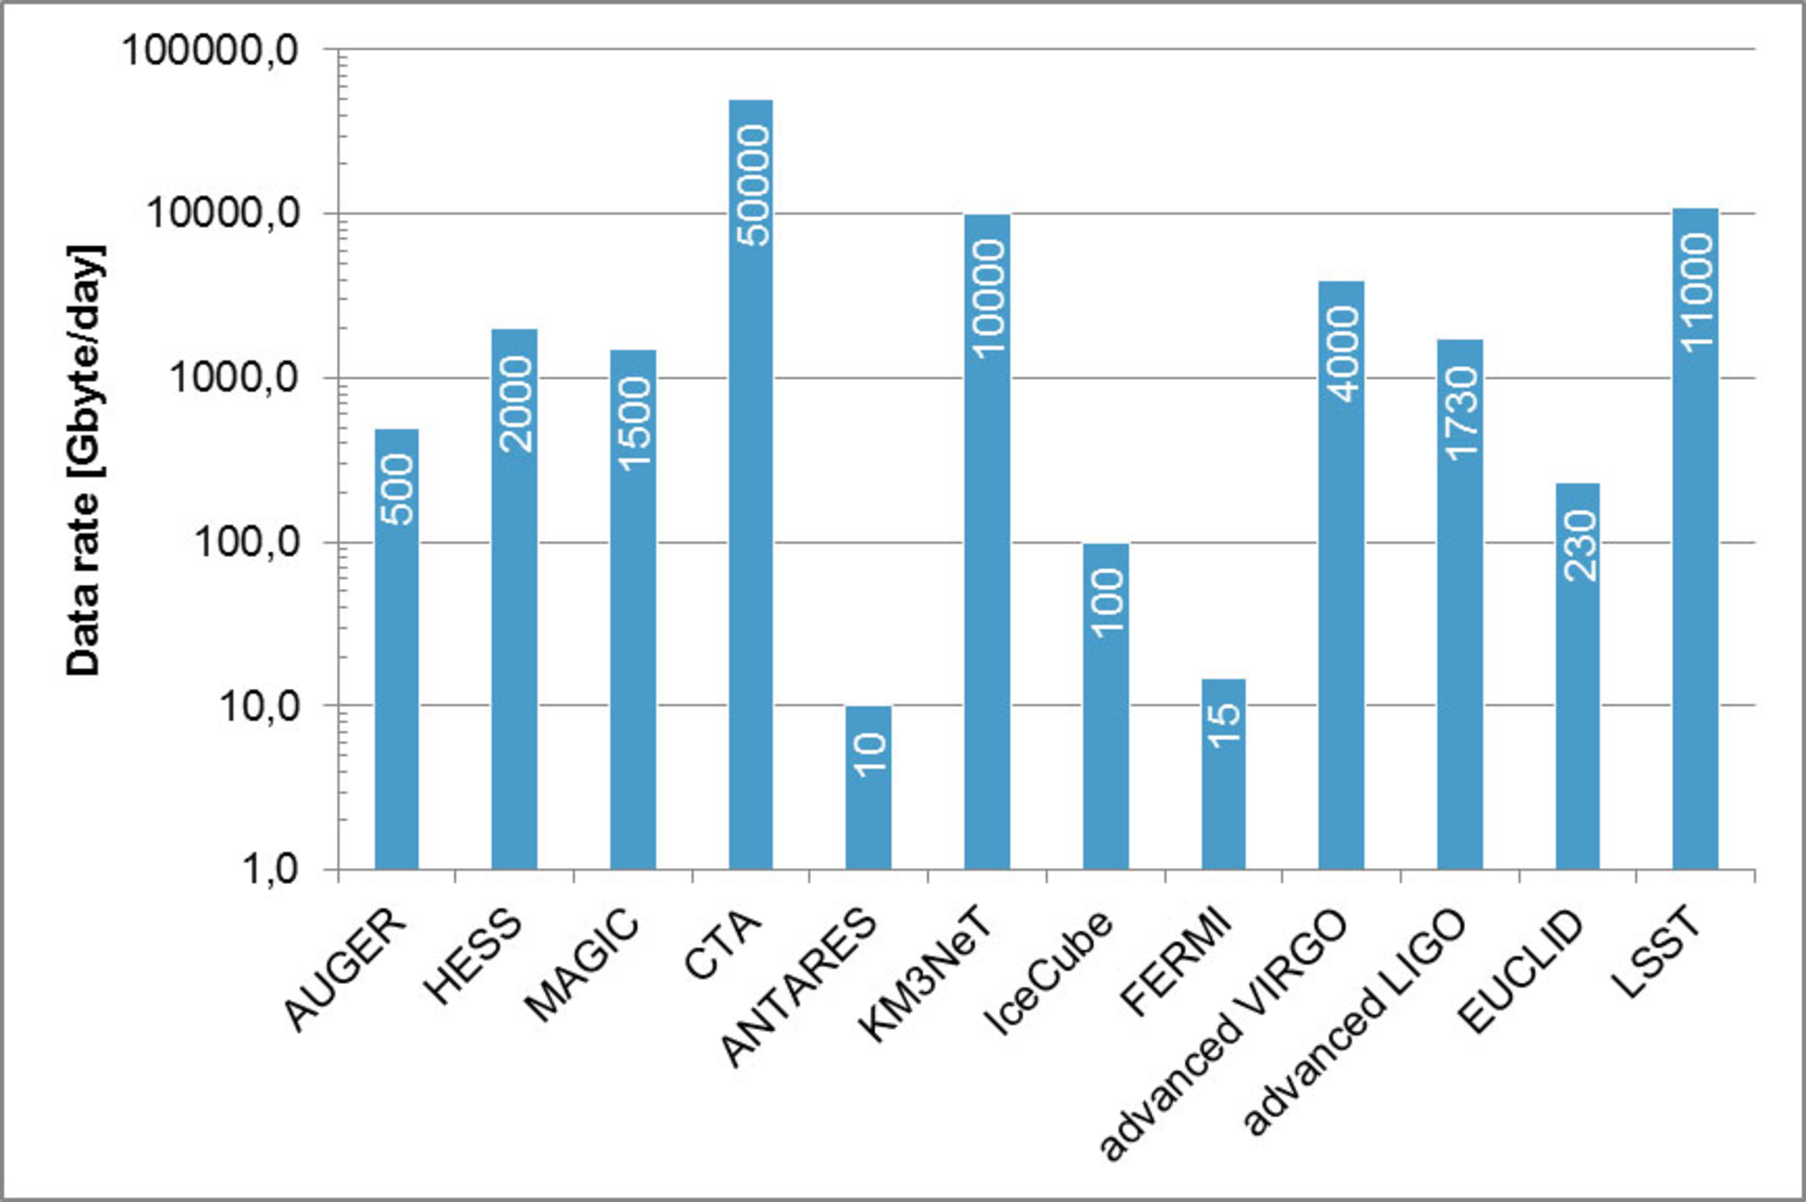
\includegraphics[width=1\textwidth]{pics/appec_computing-diagram.pdf}
        \end{center}
        \vspace{-2\parsep}
        \small Modern astroparticle experiments data rate [Gbytes/day]\footnotemark[1] %, source: APPEC brochure on Computing, 2016}
    \end{minipage}
    \hfill
    \begin{minipage}[c]{0.41\textwidth}
        \begin{itemize}
            \setlength{\itemsep}{0pt}
            \item Wide range of experiments;
            \item More than hundred years of cosmic particle measurements;
            \item Looking at the same sky with different detectors;
            \item Common data rate for astroparticle physics experiments all together is a few PBytes/year, which is comparable to the current LHC output\footnotemark[1]
            \item Big data for deep learning
        \end{itemize}
    \end{minipage}
    \footnotesize\footnotetext[1]{Berghöfer T., Agrafioti I. et all. Towards a model for computing in European astroparticle physics, Astroparticle Physics European Coordination committee, 2016}
\end{frame}

\begin{frame}{Software data life cycles}% and information management
    \begin{itemize}
        \item \textbf{Data engineering} includes development and support of data architecture and a data pipeline for a platform that enables data analysts, scientists, and other personnel to query the data.
        % and organization and support of a data pipeline that connects all the pieces of the data ecosystem together.
        
        \item \textbf{Data Life Cycle (DLC)} is the sequence of stages that a particular unit of data goes through from its initial generation 
        or capture to its eventual archival and/or deletion. The typical data life cycle includes data gathering, processing, storage, analysis, sharing and archiving. 
        % The data life cycle provides a high level overview of the stages involved in successful management and preservation of data for use and reuse.

        % \item \textbf{Data engineering} includes development of the architecture for a data platform that enables data analysts, scientists, and other curious 
        %  types to query their data and organization and support of a data pipeline that connects all the pieces of the data ecosystem together.
        %  
        %  \item \textbf{Data Life Cyce (DLC)} is the sequence of stages that a particular unit of data goes through from its initial generation 
        % or capture to its eventual archival and/or deletion. The typical data life cycle includes data gathering, processing, storage, analysis, sharing and archiving. The data life cycle provides a high level overview of the stages involved in successful management and preservation of data for use and reuse.
    \end{itemize}
    \vspace{-1ex}
    \centering
    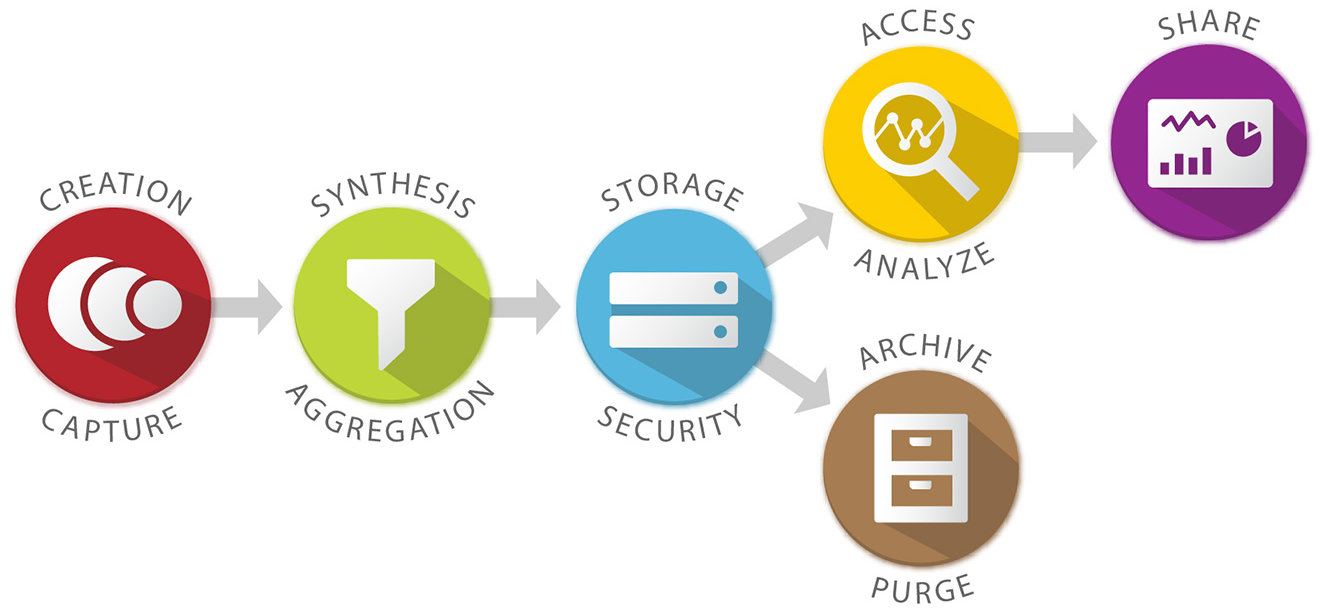
\includegraphics[width=0.65\textwidth]{pics/data_lifecycle_illust.jpg}
\end{frame}

%contents
\begin{frame}{Data engineering in APP}

\begin{minipage}[c]{0.52\textwidth}
\small
  \begin{itemize}
      \setlength{\itemsep}{0pt}
%       \item  Introduction \textcolor{kit-green100}{$\rightarrow$ we are here}
      \item  GRADLC initiative and main objectives
      \item  Features of DLC in APP
      \item  KASCADE Cosmic-ray Data Center
      \item  Proposed DLC architecture
      \item  Data aggregation server: metadata, data summary and workflows
%       \begin{itemize}
% 	  \item Metadata architecture
% 	  \item Data workflows 
% 	  \item Data summary and challenges (no slide so far :-( )
% 	  \item Possible solutions (postgres, cvmfs, etc...)
%       \end{itemize}
      \item   Application server: conception, computing sources and analysis
%       \begin{item}
% 	  \item conception 
% 	  \item computing sources
% 	  \item analysis 
% 	  \item possible solutions
%       \end{item}
      \item  Example: stacked analysis of high-energetic gamma rays
      \item  Outlook
%     \item  DCL in APP - specific
%     \item  DCL architecture
%     \item  Experiments and data specific
%     \item  Joint analysis scheme
%     \item  Possible solutions
%     \item  Outlook and future work
  \end{itemize}
\end{minipage}
\hfill
\begin{minipage}[c]{0.47\textwidth}
  
\includegraphics[width=1\textwidth]{pics/DE_fun.pdf}
\end{minipage}
\end{frame}

%GRADLC initiative descripton 

\begin{frame}{German-Russian Astroparticle \\Data Life Cycle Initiative\footnotemark[1]}
\vspace{-1.4em}
\begin{center}
  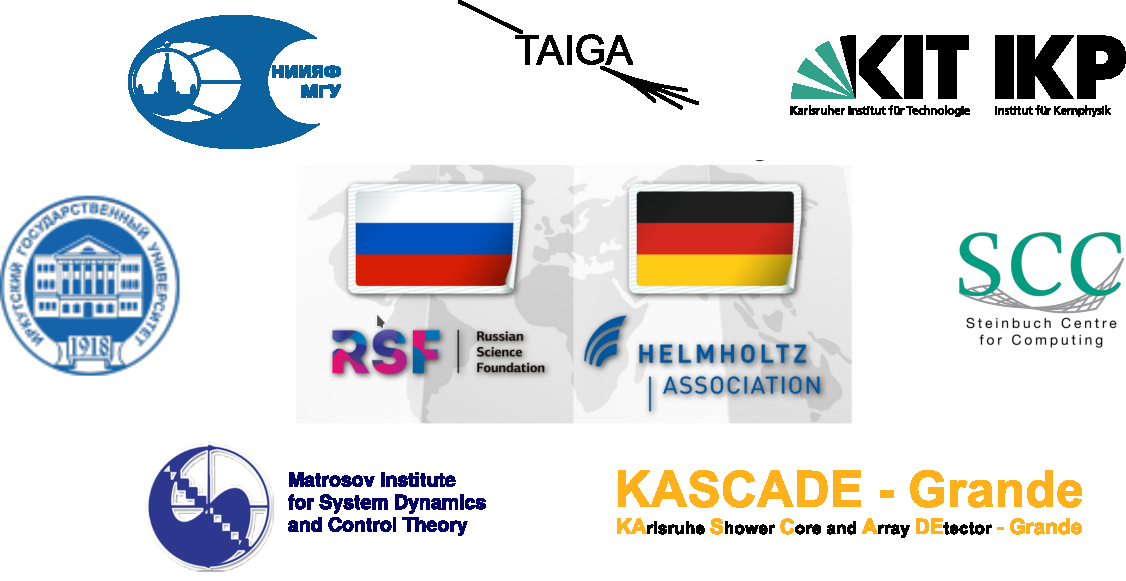
\includegraphics[width=0.9\textwidth]{pics/Collab-4.pdf}
\end{center}
\footnotesize\footnotetext[1]{Granted by RSF-Helmholtz Joint Research Groups}
\end{frame}

% %experiments overview

\begin{frame}{KASCADE-Grande}
\begin{itemize}
  \item Proposed in 1989---disassembled in 2013;
  \item Aimed at studying
  high-evergy (galactic) cosmic rays by observing extensive air showers (EAS);
%   processes at the edge of the Galaxy and beyond by observing extended atmospheric showers (EAS);
  \item Consisted of:
  \begin{itemize}
    \item scintillator arrays:
%     detecting $e$, $\gamma$, $\mu$:
    \begin{itemize}
  %сцинтиляторы, различают e, gamma, mu
    \item KASCADE---256 stations;
    \item GRANDE---37 stations;
    \end{itemize}
 %один большой калориметр
    \item Hadronic callorimeter;
 %радиодетектор
    \item Digital radio array LOPES;
%     detecting $e$, $e^{+}$;
% позволяющих наблюдать различные компоненты ливня
  \end{itemize}
  \item Important features of cosmic-ray spectrum have been obtained. The data analysis is ongoing;
%  благодаря данным с эксперимента было открыто много всего ополезного, при этом анлиз данных продолжается. новые статьи выходят
  \item KCDC (\textbf{K}ASCADE \textbf{C}osmic Ray \textbf{D}ata \textbf{C}enter, \textcolor{blue}{\texttt{http://kcdc.ikp.kit.edu}}) is a dedicated portal where all the data collected are available online. % At the moment
\end{itemize}

\begin{tikzpicture}[remember picture,overlay]
  \node[xshift=-12ex,yshift=-21ex] at (current page.north east){%
    
\includegraphics[width=0.3\textwidth]{pics/KCDC-Logo.png}
  };
\end{tikzpicture}
% \parbox[t][0pt]{0pt}{
%   \vspace{-0.63\textheight}
%   ~\hspace{0.68\textwidth}
\includegraphics[width=0.3\textwidth]{pics/KCDC-Logo.png}
% }
\end{frame}

\begin{frame}{TAIGA - Tunka Advanced Instrument for cosmic ray physics and Gamma Astronomy}
% \footnotesize
% % \vspace{-1em}
\begin{itemize}
 \item The detectors construction started in 90s with Tunka-25 setup;
 \item Changed name from Tunka to TAIGA;
 \item Is ongoing and continiously enhancend;
%  \item Currently consists of 4 detectors presented + TUNKA IACT is under construction;
\end{itemize}

% \vspace{2em}

\begin{center}
    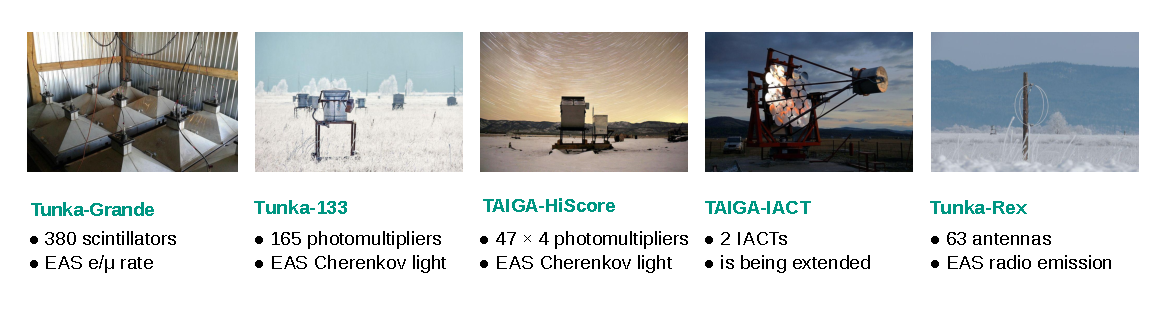
\includegraphics[width=1\textwidth]{pics/TAIGA_exp_wt.pdf} 
\end{center}

\end{frame}

 - experiments overview. Is not requiered is this IT=specified presentation
% 
% \begin{frame}{The main objectives}
% \begin{minipage}[c]{0.45\textwidth}
%   \begin{itemize}
%     \item  Provide sustainable access to scientific data
%     \item  Archiving of Data and Metadata
%     \item  Providing analysis tools
%     \item  Education in Big Data Science
%   \end{itemize}
% \end{minipage}
% \hfill
% \begin{minipage}[c]{0.54\textwidth}
%   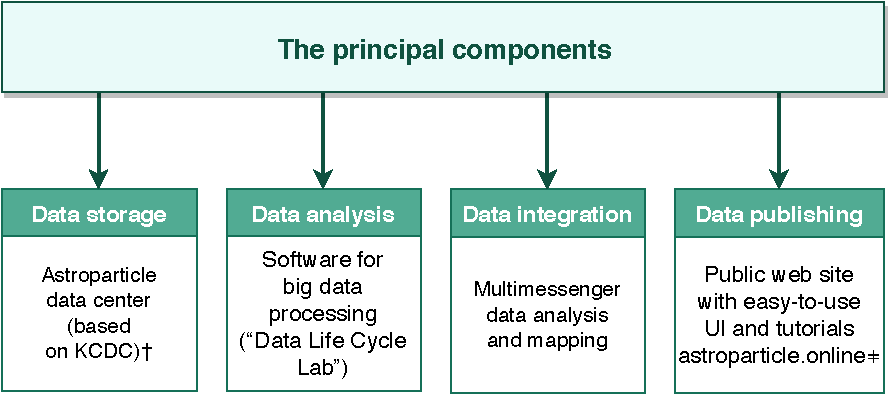
\includegraphics[width=1\textwidth]{pics/proj_objectives.pdf}
% \end{minipage}
%   \vspace{-\topsep}
%   \vspace{-\partopsep}
%   \vspace{\itemsep}
%   \vspace{\parsep}
%   \begin{itemize}
%     \item  Development area for multi-messenger analyses (e.g. Deep Learning)
%     \item  Platform for communication and exchange within Astroparticle Physics
%   \end{itemize}
% \end{frame}
% 

